\documentclass{article}

%%%%%%%%%%%%%%%%%%%%%%%%% Packages %%%%%%%%%%%%%%%%%%%%%%%%%
\usepackage[utf8]{inputenc}

\usepackage{geometry}
\geometry{left = 25 mm, top = 25 mm}%pour les marges

\usepackage{amsfonts}
\usepackage{amssymb}
\usepackage{amsmath}
\usepackage{amsthm}
\usepackage{multicol}
\usepackage{diagbox}
\usepackage{hyperref}

\usepackage{xcolor} % for setting colors

\usepackage{mathtools}
\DeclarePairedDelimiter\ceil{\lceil}{\rceil}
\DeclarePairedDelimiter\floor{\lfloor}{\rfloor}

\usepackage{array}
\newcolumntype{C}{>{\(\displaystyle}c<{\)}@{}} 
\newcolumntype{L}{>{\(\displaystyle}l<{\)}@{}} 
\newcolumntype{R}{>{\(\displaystyle}r<{\)}@{}}


%%%%%%%%%%%%%%%%%%%%%%%%% Macros %%%%%%%%%%%%%%%%%%%%%%%%%
% mathbb for class of numbers macro.
\newcommand{\BB}[1]{\mathbb{#1}}

% Integral macro.
\newcommand{\intt}[4]{\displaystyle\int_{#1}^{#2}#3\;\text{d}#4}
% use :$\intt{a}{b}{f(x)}{x}$

% end line
\newcommand{\n}{\\ [6pt]}



%%%%%%%%%%%%%%%%%%%%%%%%%%%%%%%%%%%%%%%%%%%%%%%%%%%%%%%%%%%%
%%%%%%%%%%%%%%%%%%%%%%%%% Document %%%%%%%%%%%%%%%%%%%%%%%%%
\begin{document}

%%%%%%%%%%%%%%%%%%%%%%%%% Page titre %%%%%%%%%%%%%%%%%%%%%%%
\begin{titlepage}
  \centering
  
  \rule{\textwidth}{0px}
  \vspace{15mm}
  
  \Huge{Rapport} \\
  \vspace{5mm}
  \Large Bases de données \\
  IFT 2935
  
  \vspace{40mm}
  \large par \\ \vspace{3mm}
  Zakary Gaillard-Duchassin\\ \vspace{3mm}
  Mohammed Aiman Rahmani \\ \vspace{3mm}
  Mathieu Dominique Lucien Loron \\ \vspace{3mm}
  Farley Jeannis \\ \vspace{3mm}
  Samuel Argeris \\ \vspace{3mm}
  \vspace{30mm}
  présenté à \\ \vspace{3mm}
  Jihene Rezgui
  
  \vfill
  12 mars 2024 \\ \vspace{3mm}
  
\includegraphics[scale=0.55]{logo-udem.png}
\end{titlepage}
\newpage

%%%%%%%%%%%%%%%%%%%%%%%%% Contenu %%%%%%%%%%%%%%%%%%%%%%%%%%
\section{Introduction}

\newpage
\section{Modélisation}

\subsection{Modèle Entité-Association}
\begin{center}
  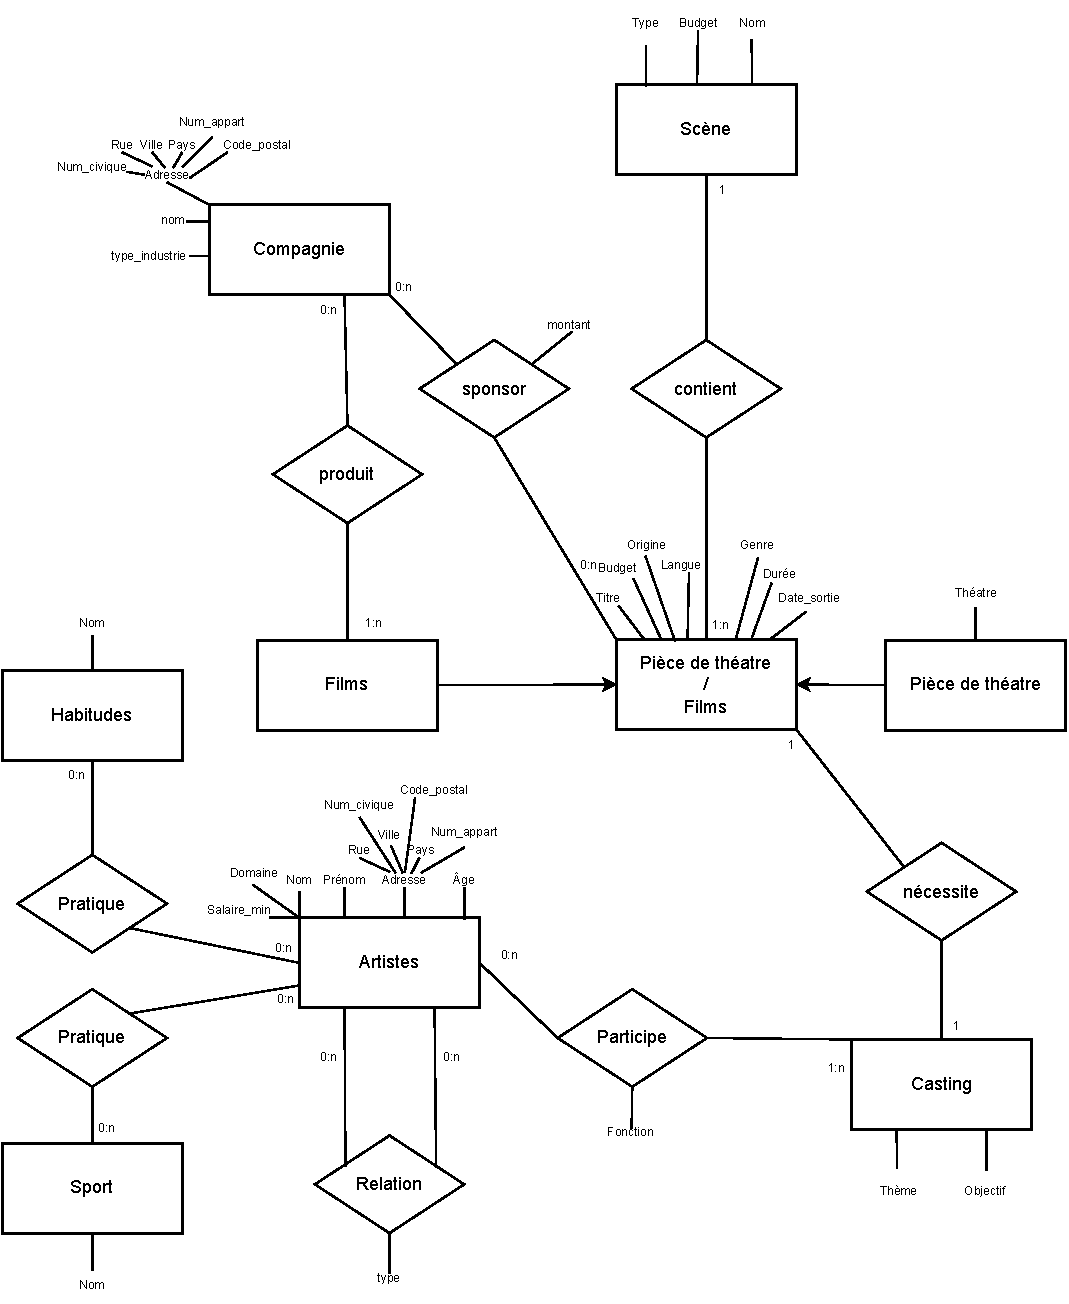
\includegraphics[scale=0.85]{../modeleEA.pdf}
\end{center}
\newpage

\subsection{Modèle Relationnel}
\begin{itemize}
\item \textbf{Oeuvre}(\underline{id\_oeuvre}, titre, budget,
  date\_sortie, durée, origine, langue, genre)
\item \textbf{Films}(\underline{\#id\_oeuvre}, \#id\_Studio)
\item \textbf{Pièces\_Théâtre}(\underline{\#id\_oeuvre}, théâtre)
\item \textbf{Scènes}(\underline{id\_scène}, titre, budget, type,
  \#id\_oeuvre)
\item \textbf{Adresses}(\underline{id\_adresse},no\_civique, rue,
  ville, code\_postal, pays, no\_appartement)
\item \textbf{Renseignement\_Supplémentaire\_Artiste}(
  \underline{id\_renseignement}, habitudes, sports, relation)
\item \textbf{Artistes}(\underline{id\_artiste}, nom, prénom,
  date\_naissance, salaire\_min, domaine, \#id\_adresse,
  \#id\_renseignement)
\item \textbf{Casting}(\underline{\#id\_oeuvre}, objectif, thème)
\item \textbf{Compagnies}(\underline{id\_compagnie}, nom,
  type\_industrie, \#id\_adresse)
\item \textbf{Sponsors}(\underline{\#id\_oeuvres \#id\_compagnie},
  montant)
\item \textbf{Producteurs}(\underline{\#id\_oeuvres
    \#id\_compagnie})
\item \textbf{Travail\_Artiste}(\underline{\#id\_artiste
    \#id\_oeuvre}, rôle, salaire, date\_début, date\_fin)
\end{itemize}


\end{document}
